\documentclass{IEEEtran}

\usepackage{amsmath}
\usepackage{listings}
\lstset{
    basicstyle=\small\ttfamily,
    breaklines=true
}
\usepackage{graphicx}
\graphicspath{ {./images/} }
\usepackage{xcolor}
\pagecolor[rgb]{0.1,0.1,0.1}
\color[rgb]{1,1,1}

\title{Readings about Sleep Tracking}
\author{Diego Linares and Eduardo Castro}

\begin{document}
  \maketitle
  \section{How Do We Sleep}
    \subsection{Introduction}
      Short and long sleep are associated with diseases such as obseity, diabetes, hypertension, etc. 7 to 9 hours is the recommended amount of time for adults, but only 40\% of the Western population achieve this, not counting quality of sleep, such as continuity, and timing, especially regarding the \textbf{circadian cycles}. \par
      The study focuses in the role of bedtime and sleep consistency as contributors to sleep quality with data from the Oura ring, which is scientifically validated.
    \subsection{Study}
      Three categories, first of 9333 people, the second of a sub-sample of those (2170 \textit{very good sleepers}). The third was a single person to provide an example of sleeping variations compared to an average \par
      The metrics considered were the following:
      \begin{itemize}
        \item Overall sleep duration
        \item Consistency of time spent in bed vs. sleep efficiency
        \item Consistency of time in bed vs. total sleep.
      \end{itemize}
      \par Sleep efficiency being the ratio of total sleep duration compared to the time in bed. In terms of consistency, we consider the difference between 75th and 25th percentile. \par 
      A \textit{very good sleeper} is a term given by the Oura ring app, with a sleep score $\geq 85$ which is based on total sleep time, efficiency, REM and deep sleep, latency and timing (circadian clock). \par 
      For these, we studied what characteristics gave them their quality sleep, especially their consistency of the bedtimes. \par 
      And for the single sleeper, a study over 587 determined his consistency between the percentiles.
    \subsection{Results and Discussion}
      \subsubsection{Population Based}
        To be included in the population you needed at least 10 nights with Oura, and the sample included $\geq 10^6$ nights. \par 
        We obtained a normal distribution of sleep with most users sleeping less than 7 hours (more than the 40\% stated in the initial questionnaire). Reasons are:
        \begin{itemize}
          \item Optimistic self-assesment.
          \item Questionnaires do not distinguish between time in bed and sleep time.
          \item Sleep tracker users sleep less than the normal population.
        \end{itemize}
        \begin{center}
          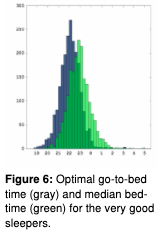
\includegraphics[width=0.20\textwidth]{sleepDistribution.png}
        \end{center}
        \par In all percentiles of sleep, there is inconsistency correlated with longer sleep times. There also seems to be a negative correlation of sleep efficiency with consistency throughout the data. \textbf{Lack of sleep consistency was found to correlate with shorter sleep duration and efficiency}.
      \subsubsection{Very good sleepers}
        They sleep an average 7.35 hours, but they \textbf{should} go to sleep half an hour earlier for best sleep quality. Half of them were also consistent sleepers. \par 
        Only 23\% of the population were considered under this. There is a relaiton between sleep quality and consistency.
      \subsubsection{Single person}
        The subject was normally consistent with his bedtime (1.2 hour difference between 25th and 75th percentile). Approx median at 22:40. There also seem to be a high correlation between late bedtime and lower sleep score.
    \subsection{Conclusion}
      Sleep is essential for humans to survive everyday challenges. Bad sleep limit our capabilities, but thanks to sleep trackers we are taking care of their effects. \par 
      With the data collected by the Oura ring, we noticed most of them were having insufficient sleep. And lack of consistency correlates with shorter sleep and lower efficiency. Next studies want to take into account other demographic factors.
  \section{Harnessing the Web for Population-Scale Physiological Sensing}
    \subsection{Introduction}
      Cognitive performance is crucial for productivity, it varies throughout the day, and it decreases after sleep loss. 150 billion dollar cost in productivity. \par 
      Models related to cognitive performance rely typically on representing:
      \begin{itemize}
        \item Circadian rhythms
        \item Homeostatic sleep pressure (more time awake means more tired)
        \item Sleep Inertia (dizziness after waking up)
      \end{itemize}
      \par Studies of these are highly artificial and controlled, and that also influences them. So they fail to account for a lot of factors, which are not well understood. 
      \subsubsection{This Work}
        The study is enabled \textit{through regraming everyday interactions with a web search engine as a aseries of performance tasks}. Such as keystrokes and clicks can show the influence of sleep in performance. \par 
        $\geq 3000000$ nights were tracked, $31000$ users, with $18$ months and $75000000$ measurements. Biggest study to date. \par 
        Performance gets to its lowest during the regular bedtime (by 31\%), but it varies depending on chronotype. \par 
        Performance is influenced by time of the day, time since waking up and a little bit by the sleep time. (23, 19 and 5 percent). \par 
        Consistent bad sleep can influence as much as 7\% in performance. \par 
        Human performance cna be monitored through patterns of interactions with devices. Which can help further work.
    \subsection{Related Work}
      \subsubsection{Circadian Processes in Sleep and Peformance}
        Daily rhythms in human performance (alertness, attention, memory, etc.), which are determined by the circadian ryhthm and the homeostatic sleep drive. Both counteract each other establishing a single consolidated period of wakefulness throughout the day. A third process is \textbf{sleep inertia}, which is the impairment after waking up. \textit{Ultradian rhythms} are shorter 90 minute ocurrences of NREM and REM stagers dudring sleep.\par 
        Chronotypes are the tendencies for sleep, and cognitive performance depend on it. Sleep deprivation might reduce performance leading to real life risks. \par 
        Some recent studies are too biased or have too small of a sample to be trusted.
      \subsubsection{Technology Use and Interaction Patterns}
        Interaction patterns have been used in small scale to understand mobile usage, stress, etc. And in large scale for insights on human behaviour, like mood rhythms.
      \subsubsection{This Work}
        Existing research is small scale or lab-based, or has subjective measures. Web search engines serve as a way to take cognitive measures. This is the largest study of objetively measure of sleep and real life performance.
    \subsection{Dataset}
      75 million interactions from $\geq 31000$ users, who use Microsoft products, especially Health app for demographic purposes. A predominantly male sample.\par 
      \subsubsection{Performance}
        Measured through the individual keystrokes for the search, and time to click on a page after the results come up. Mobile devices are excluded.
      \subsubsection{Sleep}
        Since it comes from wearable devices it is more accurate, in this case a Band, which uses proprietary algorithms. Time in bed can be inputed by the user or detected by the device. Only measurements $4 \leq x \leq 12$ hours are accepted.\par 
        They match published sleep estimates, so they are valid, it decreases with age.
    \subsection{Performance Measures Based on Interactions During Search}
      There are 2 human performance measures, which show variations based on the time and chronotype. 
      \subsubsection{Performance Measures}
        \begin{itemize}
          \item \textbf{Keystroke Time:} It is measured by the search box, it is extremely sensible since the average is 50 words per minute.
          \item \textbf{Click Time:} Time to click on a search result, excluding the ones higher than 2 minutes. 
        \end{itemize}
        \begin{center}
          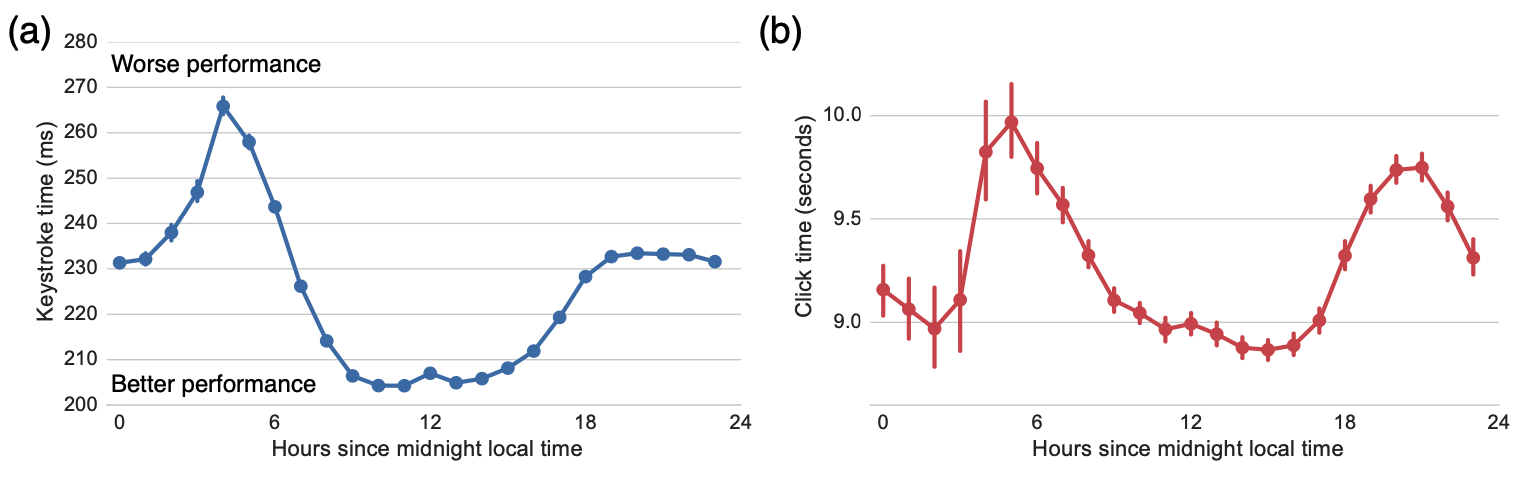
\includegraphics[width = 0.48\textwidth]{keystrokeClick.png}
        \end{center}
        \par Allows a more robust analysis, since they rely on reflexes, memory, etc. Highly relevant to many occupations. \par 
        Measurements taken on the server side, but there is no impact from network latency, because there is no much difference between requests.\par 
        Performance variation in the weekend is similar to variation during the week, so we do not consider it. Alternative performance measures (such as backstroke) are also considered.
      \subsubsection{Temporal Variation of Keystroke and Click Times}
        We validate by comparing with some smaller studies. We know that performance follows circadian rhythm. Both keystrokes and clicks follow a similar pattern throughout the day. Slowest during normal sleep time. , and the variation is around 12\% to 31\% \par 
        So these can be used to study sleep perforamnce, and can be collected non intrusively.
      \subsubsection{Performance Variation by Chronotype}
        Genetic based, determines the individual to sleep at a particular time of the day. Also affects performance. It can be determined based on \textit{Mid sleep Point on free days (MSF)}, which is the point between sleep and waking up. Formula is: 
        $$MSF_{SC}=MSF-0.5(SD_{F}-(5*SD_W+2*SD_F)/7)$$
        \par $SD$ stands for sleep duration in free and week days. The value tends to be around 4.70. \par 
        The keystroke speed varies depending on the chronotype but is between 4 and 7 am. We obtained millions of measurements of each.
    \subsection{Modeling Performance}
      We want now to make a \textbf{conceptual model of sleep} based on chronobiology. It considers circadian rhythms, homeostatic sleep drive, inertia and duration. 
      \subsubsection{Conceptual Model}
        Keystroke and click timing are based on:
        \begin{itemize}
          \item Time of the day
          \item Time in hours after wake up. 
          \item Sleep Duration in the previous night.
        \end{itemize}
        The first two are kind of correlated, and are challenging to disentangle. In laboratory this is done by sleep deprivation. In our case it is done with mathematical modeling with the millions of observations, due to the combination of usual and unusual sleep times. \par 
        \textbf{Potential Confounding Factors:} In keystrokes we take into the account the exact character typed since some take longer than others, and in clicks, results on the bottom take longer. \par 
        Navigational queries have fast clicks, while informational ones take much longer (@ seconds). So this has to be taken into account. \par 
        Another way of doing it is to compare click times for exactly identical queries (popular ones mostly). \par 
        Repeated queries also yield faster performance, but only 4\% of them fall under this category. 
      \subsubsection{Mathematical Formulation}
        This is the model for keystroke timing. Considering fixed and additive effects.
        $$y_i=\alpha+f^k(x^k_i)+f^t(x^t_i)+f^w(x^w_i)+f^d(x^d_i)+\epsilon_i$$
        \par $y_i$ being keystroke time, the upper index of $f$ are the functions of interest (type, time of day, time since wake up, sleep duration) and their output features, with $\epsilon$ being residual. \par 
        Function spaces are discretized (something like "between 0 and 15 mins since waking up"). Functions are then denoted to their respective bins, and the discretized features are mapped to a constant value, and it becomes a much more complex model.
      \subsubsection{Results}
        We have 3 functions $c^t,c^w,c^d$ which model the impact of time of day, time since wake up and sleep duration. The function results \textit{in the paper} are very similar and smooth.
        \begin{itemize}
          \item \textbf{Time of Day:} Varies and it is slowest at 4 am. Then it improvees and it goes down at around 7 pm. Which fits the circadian rhythms. The variations for keystrokes and clicks are 40 miliseconds and 2.1 seconds (18 and 23\%).
          \item \textbf{Time after Awakening:} In this case we see 42 miliseconds for keystrokes (19\%) and 1.6 seconds (1.7\%) for clicks. As sleep inertia leaves, time rapidly improves. Until 16 hours after being awake, performance goes down again as it is sleep time. Keystrokes are more stable.
          \item \textbf{Time in Bed:} Variation is much smaller, 12 miliseconds and 0.25 seconds (5\% and 3\%). But we can see that sleeping too little or much can decrease performance. Forms an U shaped relationship.
        \end{itemize}
    \subsection{Influence of Insufficient Sleep on Performance}
      In this case we add some of the laboratory research in our study.
      \subsubsection{Single Nights of Insufficient Sleep}
        Significantly slower when in bed for less than 6 or more than 9 hours. With increases of 4\%. \par 
        Sleeping earlier has no much impact, but sleeping more than an hour late can cause increases of 7.3\% longer keystrokes. And this is not only on weekends (less pressure) but also with weekday data. \textbf{Sleeping later in one's circadian cycle does not satisfy the neural recovery needed for proper daytime performance}.
      \subsubsection{Multiple Nights of Insufficient Sleep}
        We consider 3 different scenarios:
        \begin{itemize}
          \item Two nights of sleep with more than 6 hours each (SS)
          \item One night over and the next night with less than 6 hours (SI)
          \item Two nights in a row with insufficient (II)
        \end{itemize}
        This is considered for a week and reduced for a single value. Sleep patterns not taken into account. We also dont control sleep \textbf{preceding or following} the control nights, to check real world impact of the sleep loss. \textbf{Recovery time} is the time necessary to reach performance similar to the one of two regular sleep nights. \par 
        \textbf{Results:} 1.2\% worse performance after one bad night, and 4.8\% after two bad nights. Even taking into account compensation chemicals such as increased caffeine intake. It takes 3 nights to recover from one insufficient night of sleep, and six to recover from two. \par 
        Since we don't control days prior and after, we must check if these contribute to the recovery time in the future, usually insufficient sleep nights are followed by more and more bad sleep nights. 
    \subsection{Conclusion}
      Sleep is critical to productivity learning and safety. It exhibits variations throughout the day. This is a large study necessary to advance our understanding of this. \par 
      \subsubsection{Summary of Results}
        400 times the number of subjects of the largest study to date. We used info from a web engine use and wearable devices. Results agree with lab ones, and we desgined a statistical model. Quantified periods of lower performance. \par 
      \subsubsection{Implications}
        We dont need to do explicit testing on humans. Performance varies throughout the day based on chronotype and sleep. There is great potential in harnessing online activities to monitor motor skills, cognition, etc.
        \begin{itemize}
          \item We can do studies outside a small lab.
          \item Non intrusive measurement of cognitive performance.
          \item Much more realistic measures, and continuous monitoring
        \end{itemize}
        \par This can even be used to adapt user experience appropriately. 
  \section{Sleep Debt in Student Life}
    \subsection{Introduction}
      Sleep is a popular topic, and how people don't get enough of it. Deprivation of it can lead to workplace mistakes, accidents, etc. We want to explore how it affects how people use \textbf{IT}. \par 
      Since students and info workers are available mosts of the day and night, IT and sleep are closely related, and how the former might disrupt or shorten sleep. \par 
      Human-Computer Interaction (HCI) has checked new ways of measuring sleep. Also, there are not too many studies on how \textit{sleep affects IT use} (the converse). Is important as sleep could be considered as a variable in HCI research, and find what computer behaviours happen when the user lacks sleep, and find interventional ways to improve sleep through tech. \par 
      This study is \textit{in situ}, focused on students. Results show that with less sleep you perceive higher pressure and productivity, but spend more time on Facebook. 
      \subsubsection{Sleep and Information Technology Use}
        \textbf{Sleep Duration and Performance:} Negative cognitive and health outcomes. 37\% of adults suffer from it, and "evening types" suffer emotional and attention problems. \par 
        \textbf{Sleep Debt:} Cummulative loss and pressure for sleep. Can come from many sources. It is directly related to the daily need of sleep. \par 
        \textbf{College Students and Sleep Durations:} Very common, more in women, and has impact on scores. Sleep disturbances might come from the use of IT, since it stretches the evening. \par 
        \textbf{Sleep and Social Media Use:} Same as before, staying late to do stuff in social media. It requires less effortful thinking, so tired students might prefer this to more difficult tasks. \par 
        \textbf{Sleep and Multitasking:} You tend to multitask less with better sleep. Since you have less atteention with lack of sleep. This is due to what is known as self-interruptions. 
      \subsubsection{Research Questions}
        Again, we look at the converse, how sleep deprived people use IT. We mostly examine sleep duration the night before and the sleep debt with different variables. The research questions are:
        \begin{itemize}
          \item \textit{What are the impacts of sleep on college students' perceptions of productivity and work pressure?} So we want to know if less sleep is associated with higher subjective work pressure and lower perceived productivity.
          \item \textit{Is sleep related to college students' multitasking on the computer?} Decreased sleep reduces attention and focus, then with less sleep you have higher multitasking, because you don't have as much attention on the computer screen. 
          \item \textit{Is sleep debt associated with Facebook use?} Social media is seen as a lightweight task, needed to stay connected. We expect changes over cummulative sleep loss. When you are tired you do tasks with less cognitive resources, so Facebook comes as both as relaxing activity and distraction.
          \item \textit{How is sleep debt related to mood?} Negative impact has been studied before, but only in long periods of deprivation. So sleep debt is the one to be taken into account.
        \end{itemize}
    \subsection{Methodology}
      Large University during various months in 2014. Mixed method approach with computer logging and surveys to obtain data.
      \subsubsection{Participants and Procedure}
        76 undergraduates, with a mean of 19 years. They got logging software installed, and were sent 2 daily surveys. One week in, interviews were conducted.
      \subsubsection{Measures}
        71 people gave proper data. \textit{Kidlogger} was used to see how they switched through tabs and such. Time spent in each app (not idle) was counted. Idle time was counted with AWARE framework. 
        \begin{itemize}
          \item \textbf{Facebook Measures:} Obtained from computer and phone logs to obtain a total daily time on it. 
          \item \textbf{Focus duration:} Can be depending on task switching between the same app or switching between apps. But we consider the second. We measured average duration spent on any active window.
          \item \textbf{Sleep Duration:} Self report sleep diary, up to hour and minute, and seem to be very accurate and validated. 
          \item \textbf{Sleep Debt:} Usually accumulated on work days and compensated on free days. The larger the difference of sleep between the two, the larger the debt. The formula is the same we saw in the previous paper. Sleep debt tends to have a long tail so we used a log transformation to make it a normal distribution.
          \item \textbf{Mood:} PANAS scale. Which measures positive and negative effect, we substracted the latter from the former.
          \item \textbf{Survey Measures:} Quesstions about work pressure and perceived productivity, as well as some other student-related info.
        \end{itemize}
      \subsubsection{Measures Used}
        Definitions of the measures:
        \begin{itemize}
          \item Work Pressure: Likert scale (1 - 5) about how much pressure did they have today.
          \item Perceived Productivity: Same, but for how productive.
          \item Sleep Duration: Self-reported daily.
          \item Sleep Debt: Calculated with the formula, based on the values before.
          \item Total Computer Duration: Logging software detected.
          \item Focus Duration: Average time on any computer window, with one outlier removed.
          \item FB Duration: Daily time on Facebook, also removing one outlier, and square root transformed.
          \item Affect Balance: PANAS score 
          \item Interviews: Semi-structured
          \item Control variables: Age, gender, workload and deadline influence.
        \end{itemize}
    \subsection{Results}
      1720 hours were detected, participants said it wasn't intrusive.
      \subsubsection{Overview of results}
        Average sleep duration was 7.9 hours, but a range from 2.6 to 14. Positive sleep debt (negative correlated with duration $r=-0.11$). Focus duration was 1 minute, 38 seconds.
      \subsubsection{Research questions and analyses}
        Linear mixed-effects models, subjects being random effects. All other factors were fixed effects. Only used days with full data collection and when it was greater than 0. We used Satterthwaite approximation for calculating denominator degrees of freedom. 
      \subsubsection{Impacts of sleep on perception of work pressure and productivity}
        Sleep duration was negatively associated with reported work pressure the next day (less sleep, more pressure). $R^2=0.56$. Deadlines were positively correlated with work pressure. Control variables weren't significant. \par 
        Surprisingly, people reported less perceived productivity if they slept more. $R^2 = 0.17$. Deadlines were positively correlated still. \par 
        In interviews, staying late was associated with more pressure next day. Sometimes "wasting time" on technology was the reason for it. Also, longer sleep was related with a more relaxed schedule, which makes sense for the less productivity. Most of them also used less tech on weekends because they slept more.
      \subsubsection{Sleep and Computer Usage}
        Significant effect of sleep duration on Focus duration. $R^2=0.04$. And the deadline control variable was negatively correlated, the more deadlines, the less focus. \par 
        Sleep deprivation resulted in less focus. Some think using the internet for a bit helps waking up. Some just mention constant distraction.
      \subsubsection{Sleep and Facebook and Other Social Media Use}
        The bigger the sleep debt, the more time on Faacebook. $R^2=0.06$. Even with more workload and deadlines. Some interviews revealed it could be a strategy to stay awake. Some also consider it part of their sleep and awake routine. \par 
        51 reported it doing the activity to escape their schoolwork and relieve stress. Some are aware of the impact it has on their sleep.
      \subsubsection{Sleep and Mood}
        Studies from the table in the paper show that the more sleep debt, the more negative is the mood $R^2=0.1$. Females had a significant more positive mood.
    \subsection{Discussion}
      We show that sleep duration impacts IT usage. Short sleep means more pressure and perceived productivity, but with less focus. With more sleep debt, we also see more social media use, and negative mood. \par 
      Our work sheds light on the phenomenon of sleep affecting IT use and mood. \par 
      Multitasking was also an important part, and lack of sleep is related to it, because of the less focus, which is a sign of poor cognitive functioning. So it is not only caused by software factors, but also things that affect the student externally (deadlines as well). \par
      This helped to see sleep effects on performance \textit{in situ}. 
      With less sleep it is possible that students spend more time in work activities, or get more work done, so that is why the higher perceived productivity. Plus the deadlines, this correlates to higher pressure. It might have benefits, but also repercussions. \par 
      Pressure means more cognitive demands, and social media means less effort thinking, that is why people turn to it under stress. \par 
      Due to the distractions caused by less sleep, people self-interrupt more, like for Facebook. It provides a mental break. And it provides a reflection rather than a cause of less sleep. This could be tested in lab. Also not all its use is for leasure. \par 
      Behavior in social media, however, can be very diverse so not all behaviours are like Facebook, but this one is the most popular. Some different patterns might change as new social media arises. \par 
      Negative mood because of lack of sleep has been found in labs and now \textit{in situ}. \par 
      So the relation between IT and sleep is bidirectional, which is important because the variables are reciprocal. 
      \subsubsection{Designing for sleep patterns}
        Some ideas on how tech can help to remedy the effects of lack of sleep. For example, interface design, so they adapt to the individual's practices, like triggering interventions from time to time. Also, doing lightweight use of IT in the morning, can ease you up into heavy duty. Amount of sleep is gonna be a control variable in future user experience studies.  \par 
      \subsubsection{Limitations}
        We can't establish a causal relation between sleep duration the night before and sleep debt. \par 
        Facebook use might also be overestimated, especially because sometimes use is counted even when the user is asleep. \par 
        Sleep quality was not measured as well, and self-report could be changed for something more observational. \par 
        Results apply mostly to college students, but some of it can be generalized. Especially window focus.
    \subsection{Conclusions}
      Sensors and biosensors might come crucial for the HCI community. Sleep duration impacts IT usage, so it is not just a one way relation. This might spark future research into other techniques to explore the relationship.
  \begin{thebibliography}{}
    \bibitem{Koskimaki}
      \textit{How Do We Sleep - a Case Study of Sleep Duration and Quality Using Data from Oura Ring},
      Hell Koskimaki for Ubicomp / ISWC'2018 Adjunct
      From: 10.1145/3267305.3267697
    \bibitem{Althoff}
      \textit{Harnessing the Web for Population-Scale Physiological Sensing: A Case Study of Sleep and Performance}
      Tim Althoff for Conference: the 26th International Conference
      From: 10.1145/3038912.3052637
    \bibitem{Mark}
      \textit{Sleep Debt in Student Life: Online Attention Focus, Facebook, and Mood}
      Gloria Mark for 2016 CHI Conference
      From: 10.1145/2858036.2858437
  \end{thebibliography}
\end{document}